\section{Parameter-Efficient Fine-Tuning}
\label{sec:peft}

\noindent\textbf{SQ1:} \textit{What structural properties of
parameter-efficient adapters make them suitable as transmissible, composable
knowledge units in a peer-to-peer setting?} This section surveys the major
PEFT families and their structural properties to answer SQ1, which is resolved
in the centralised discussion in Section~\ref{sec:synthesis_gap:answers}.

\subsection{The Fine-Tuning Bottleneck}
\label{sec:peft:intro}

Full fine-tuning of a pre-trained transformer model updates every weight in the network
to adapt it to a target task. For models at the scale of contemporary large language models (ranging from hundreds of millions to hundreds of billions of parameters)
this approach is prohibitively expensive in terms of both storage and compute. Each
task requires a separate copy of the full model, and gradient updates of the same
dimensionality as the weight matrices must be held in memory during training. The
parameter-efficient fine-tuning (PEFT) paradigm addresses this by confining updates to a
small, structured subset of parameters while keeping the pre-trained backbone frozen
\cite{DingNature2023}. Surveys by Han et al.~\cite{Han2024} and Wang et al.~\cite{WangAIReview2024}
catalogue over thirty PEFT methods proposed between 2019 and 2024, and Mao et al.~\cite{MaoLoraSurvey2024}
systematically analyses the convergence and expressive properties of the low-rank
adaptation family. The common thread is the observation, formalised by Zeng et al.~\cite{ZengExpressive2024},
that task-specific adaptation requires updates that lie in a substantially lower-dimensional
subspace than the full weight manifold; PEFT methods exploit this structure to achieve
near-parity with full fine-tuning at a fraction of the parameter cost.

When this low-dimensionality property is combined with the frozen-backbone constraint,
each task's adapter becomes a self-contained, portable parameter set: storable, transmissible,
and composable independently of every other task's adapter and of the base model itself.

\subsection{Bottleneck Adapters}
\label{sec:peft:bottleneck}

Houlsby et al.~\cite{Houlsby2019} introduced the bottleneck adapter architecture, which inserts compact
residual modules at two points within each transformer layer: immediately after the
multi-head self-attention sub-layer and after the feed-forward network (FFN) sub-layer.
Each adapter applies a down-projection from the hidden dimension $d$ to a smaller
bottleneck dimension $r$, a non-linearity (GeLU), and an up-projection back to $d$,
with a residual skip connection so that a zero-initialised adapter leaves the model
behaviour unchanged at the start of training:

\begin{equation}
h \leftarrow h + W_\mathrm{up}\,\sigma(W_\mathrm{down}\,h)
\label{eq:bottleneck_intro}
\end{equation}



Note: Equation~(\ref{eq:bottleneck_intro}) presents a simplified form of the Houlsby bottleneck adapter.
The original Houlsby et al.~\cite{Houlsby2019} architecture additionally applies layer
normalisation to the adapter input before the down-projection, which is abstracted away in
Equation~(\ref{eq:bottleneck_intro}) for clarity. Figure~\ref{fig:houlsby_adapter} shows the full
architecture, including this normalisation step.

\begin{figure}[H]
    \centering
    % Schematic of the bottleneck adapter architecture.
    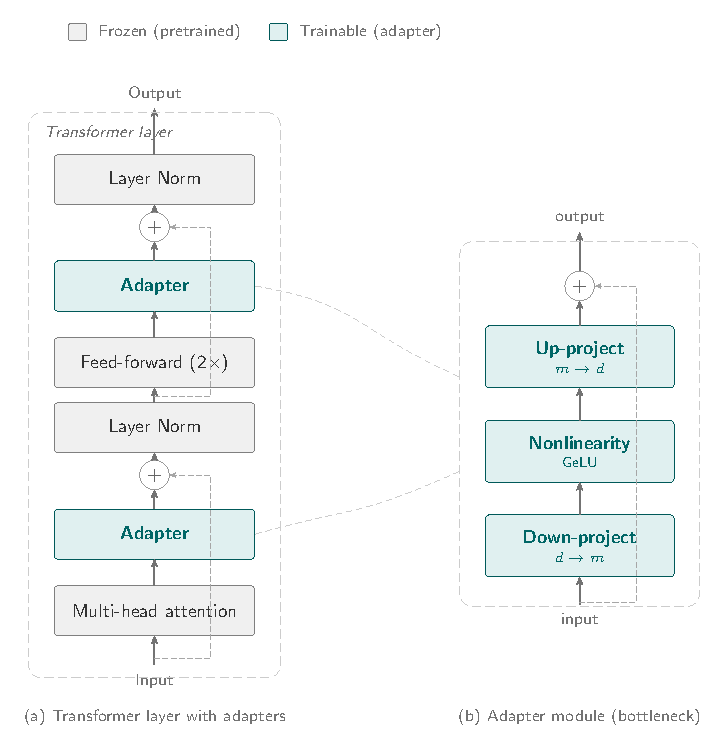
\includegraphics[width=0.8\textwidth]{figures/fig_houlsby_adapter_figure.pdf}
    \caption{Bottleneck adapter architecture (own figure)
    \cite{Houlsby2019}. (a)~A transformer
    layer with adapter modules inserted after the multi-head attention and
    feed-forward sub-layers; dashed lines indicate the residual connections that
    bypass each sub-layer--adapter pair. (b)~Internal structure of a single adapter
    module: a down-projection to bottleneck dimension $r$, a GeLU nonlinearity, an
    up-projection back to $d$, and a skip connection that initialises the module to
    an identity function at the start of training.}
    \label{fig:houlsby_adapter}
\end{figure}

\vspace{-0.5em}

where $W_\mathrm{down} \in \mathbb{R}^{r \times d}$ and $W_\mathrm{up} \in
\mathbb{R}^{d \times r}$. With $r \ll d$, each task's adapter contributes only
$2rd$ additional parameters per layer --- typically $3.6\%$ parameters
added per task on BERT
\cite{Houlsby2019}. Evaluated across 26 diverse NLP tasks,
bottleneck adapters matched full fine-tuning accuracy within 0.4\% on GLUE \cite{WangGLUE2018} while
training only this small fraction of weights.

He et al.~\cite{HeEffectiveness2021} conducted a comprehensive empirical comparison of adapter
placement strategies, demonstrating that inserting adapters after the FFN sub-layer
alone matches the dual-placement scheme while halving the added parameter count.
R{\"u}ckl{\'e} et al.~\cite{RuckleAdapterDrop2021} showed that adapters in lower transformer layers can be
dropped at inference time with minimal accuracy loss, enabling dynamic accuracy--efficiency
tradeoffs that are particularly relevant for heterogeneous inference nodes.
Poth et al.~\cite{PothAdapters2023} provided a systematic analysis of adapter capacity requirements
across task types, finding that low-resource and cross-lingual tasks benefit most from
the compact per-task parameterisation.

A key structural property of bottleneck adapters from the perspective of this review is
their modularity: each task's adapter is a self-contained parameter set, independent of
every other task's adapter, and additive with respect to the frozen backbone.
Task-specific knowledge is localised entirely within the two weight matrices
$W_\mathrm{down}$ and $W_\mathrm{up}$, enabling selective loading at inference time
without modifying the shared model state.

\subsection{Low-Rank Adaptation (LoRA)}
\label{sec:peft:lora}

Hu et al.~\cite{Hu2022} proposed Low-Rank Adaptation (LoRA), which reparameterises weight updates
as low-rank matrix products rather than inserting additional modules. For a frozen
weight matrix $W_0 \in \mathbb{R}^{d \times k}$, LoRA adds the decomposed update
$\Delta W = BA$, where $B \in \mathbb{R}^{d \times r}$ and $A \in \mathbb{R}^{r \times k}$
with rank $r \ll \min(d, k)$:

\begin{equation}
W' = W_0 + \Delta W = W_0 + \frac{\alpha}{r} BA
\label{eq:lora_intro}
\end{equation}

where $\alpha$ is a fixed scaling hyperparameter that decouples the rank $r$ from the learning rate. This decoupling allows $r$ to be changed without re-tuning the optimiser hyperparameters.

The matrix $A$ is initialised with a random Gaussian, $B$ is initialised to zero, so
the adapted model is identical to the pre-trained model at the start of training. 

At inference time, the low-rank update can be merged into $W_0$ by computing
$W' \leftarrow W_0 + \frac{\alpha}{r}BA$ (with the scaling factor $\frac{\alpha}{r}$ absorbed into the merged weights), so that adapted and base-model inference share
exactly the same computation graph with zero added latency. In the original work, LoRA targets
$W_q$ and $W_v$ by default; subsequent studies demonstrate that applying LoRA to all
projection matrices including $W_k$, $W_o$, and FFN layers is required to match full
fine-tuning performance. With $r = 4$, LoRA matches full fine-tuning on GLUE benchmarks using
RoBERTa/DeBERTa-scale models, and separately matches full fine-tuning on
generation benchmarks (WikiSQL, MultiNLI, SAMSum) at GPT-3-175B scale
\cite{Hu2022}, at a parameter overhead of
approximately 0.01\% of the original model weight count.

The theoretical basis for LoRA's effectiveness was established earlier by work on
intrinsic dimensionality and low-rank gradient structure: Zeng et al.~\cite{ZengExpressive2024}
showed that the gradient signal during fine-tuning lies near a low-rank manifold, and
that models pre-trained at scale are already close to the optimum for most downstream
distributions. This makes the low-rank constraint a descriptively accurate model of the
true update, not merely a regularisation heuristic.

Two structural properties of LoRA are worth noting beyond the accuracy numbers. The merged
representation $W' = W_0 + BA$ means that an adapted model is computationally identical to
the base model at inference time, incurring no extra latency once the matrices are combined.
Conversely, keeping $A$ and $B$ separate allows multiple per-task adapters to coexist
alongside a single frozen backbone, with task switching requiring only a matrix substitution
rather than a model reload, a property that the multi-tenant serving systems reviewed in
Section~\ref{sec:inference_systems} exploit directly.

\subsection{Advanced LoRA Variants}
\label{sec:peft:lora_variants}

\paragraph{QLoRA.}
The memory cost of keeping even a frozen backbone in full precision limits LoRA's applicability to consumer hardware. Dettmers et al.~\cite{Dettmers2023} combined LoRA with 4-bit quantisation of the frozen base model to
enable fine-tuning of 65-billion-parameter models on a single 48~GB GPU. The base model
weights are stored in 4-bit NormalFloat (NF4) format  (a quantisation scheme optimised
for the near-normal distribution of pre-trained weights) while LoRA adapter weights
remain in 16-bit precision. QLoRA further introduces Double Quantisation (quantising
the quantisation constants themselves, saving ~0.37 bits per parameter) and Paged
Optimisers (using NVIDIA unified memory to manage GPU memory spikes during
backpropagation). Combined with 4-bit quantisation, QLoRA reduces the base model memory footprint by approximately 4$\times$ compared to full 16-bit loading (e.g., from $\sim$130~GB to $\sim$33~GB for a 65B model), without degradation in adaptation quality: the
Guanaco model family fine-tuned via QLoRA reached 99.3\% of ChatGPT performance on the
Vicuna benchmark \cite{Dettmers2023}. The NF4 quantisation applies only to the frozen
backbone; the LoRA adapter matrices are kept in standard precision and are trained and
transferred independently, so the quantised backbone and the per-task adapter delta
remain decoupled artefacts with different memory and transmission characteristics.

\paragraph{AdaLoRA.}
Rather than applying a uniform rank $r$ across all weight matrices, Zhang et al.~\cite{ZhangAdaLoRA2023}
proposed AdaLoRA, which uses an SVD-like parameterisation
$\Delta W = P \Lambda Q$ with orthogonality regularisation to avoid expensive exact SVD
recomputations. This allows the effective rank budget to be concentrated in weight
matrices where the adaptation signal is strongest. AdaLoRA matches or surpasses fixed-rank
LoRA across GLUE and SuperGLUE without increasing total parameter count, and the
adaptive allocation is particularly useful when different tasks require substantially
different updates to different sub-networks.

\paragraph{DoRA.}
Liu et al.~\cite{LiuDoRA2024} proposed Weight-Decomposed Low-Rank Adaptation (DoRA), which
factorises the adapted weight matrix into a magnitude component (a scalar vector) and
a directional component (normalised weight), applying LoRA only to the directional part.
This decomposition more closely mimics the update pattern of full fine-tuning, which tends
to make large magnitude changes in early layers and directional changes in later layers.
DoRA consistently outperforms LoRA with the same rank budget on language and multi-modal
benchmarks.

\paragraph{ReLoRA.}
Lialin et al.~\cite{LialinReLoRA2023} proposed ReLoRA, which extends LoRA to the pre-training regime
by periodically resetting the low-rank factors and merging the accumulated update into the
base model, then reinitialising with a fresh low-rank decomposition. Applying ReLoRA to
models up to 350M parameters achieved comparable perplexity to full pre-training with
significantly fewer simultaneously active parameters, demonstrating that the low-rank
constraint need not be limited to the fine-tuning phase.

\subsection{Prompt-Based Adaptation Methods}
\label{sec:peft:prompt}

In parallel with the adapter and low-rank adaptation families, a distinct class of PEFT
methods conditions transformer behaviour by prepending learnable vectors to the input
sequence, rather than inserting or modifying weight matrices within the network.

Li and Liang~\cite{LiLiang2021} introduced Prefix Tuning, which prepends a set of trainable
continuous vectors (a ``prefix'') to the activation sequence at each transformer
layer as additional virtual tokens, which the attention mechanism then attends to across
both keys and values. The prefix vectors act as virtual tokens that steer the attention
mechanism without
altering any model weights; only $0.1\%$ of parameters are updated during training.
Prefix Tuning matches full fine-tuning performance on
table-to-text generation (evaluated with GPT-2 \cite{RadfordGPT22019}) and summarisation (evaluated with BART \cite{LewisBART2020})
\cite{LiLiang2021}, with separate prefix vectors for each task enabling independent
storage and selective loading at inference time.

Lester et al.~\cite{Lester2021} proposed a simpler variant, Prompt Tuning, which adds a small number
of learnable tokens only at the input embedding layer (not at every layer), making it
even more parameter-efficient. On T5-class models \cite{RaffelT52020} at 11B parameters, Prompt Tuning
matched the performance of full fine-tuning across a broad range of tasks; at smaller
scales, a gap persisted that narrowed with model size \cite{Lester2021}. The finding
that scale reduces the required capacity of the soft prompt is consistent with the general
finding that foundation-model representations are increasingly complete, making small
deltas sufficient for task conditioning.

Ben-Zaken et al.~\cite{BenZaken2022} demonstrated that fine-tuning only the \textit{bias parameters}
of a transformer network (BitFit) (approximately 0.08\% of BERT-Large's total
parameters achieves performance competitive with full fine-tuning on GLUE in small-to-medium data regimes.
BitFit requires no added modules and imposes virtually no additional memory or computation
at inference time, making it among the most transmission-efficient forms of PEFT: the per-task
parameter delta is a set of scalar bias vectors, occupying kilobytes rather than
megabytes.

\subsection{Hypernetwork-Based Adaptation}
\label{sec:peft:hypernetwork}

Bottleneck adapters, LoRA, and prompt-based methods all produce per-task parameter sets
that are trained independently and do not share information across tasks during the
training phase. Mahabadi et al.~\cite{MahabadiCompacter2021} proposed Compacter, which combines
hypercomplex multiplication layers with low-rank factorisation to generate adapter weights
from compact parameter tensors, reducing the total adapter parameter count by approximately two orders of magnitude
compared to standard bottleneck adapters (0.047\% of a full fine-tuning parameter budget).
Mahabadi et al.~\cite{Mahabadi2021} proposed HyperFormer, which uses a shared hypernetwork
to generate adapter weights conditioning on task embedding, layer identifier, and adapter
position to generate layer-specific adapter parameters, enabling explicit knowledge
sharing across tasks. HyperFormer's conditioning on all three inputs: task embedding,
layer identifier, and adapter position, means that training on one task
can inform adapter generation for related tasks without coupling the adapters' inference
behaviour.

He et al.~\cite{HeUnifiedPEFT2022} provided a unified framework showing that adapters, prefix
tuning, and LoRA can all be expressed as instances of a general \textit{modified
representation} model that adds a structured delta to some subset of the
transformer's internal representations. This unification simplifies theoretical analysis
and enables systematic comparison of the PEFT families surveyed in this section
(Figure~\ref{fig:peft_types}) along the axes of placement, structure,
and parameterisation.

\begin{figure}[H]
  \centering
  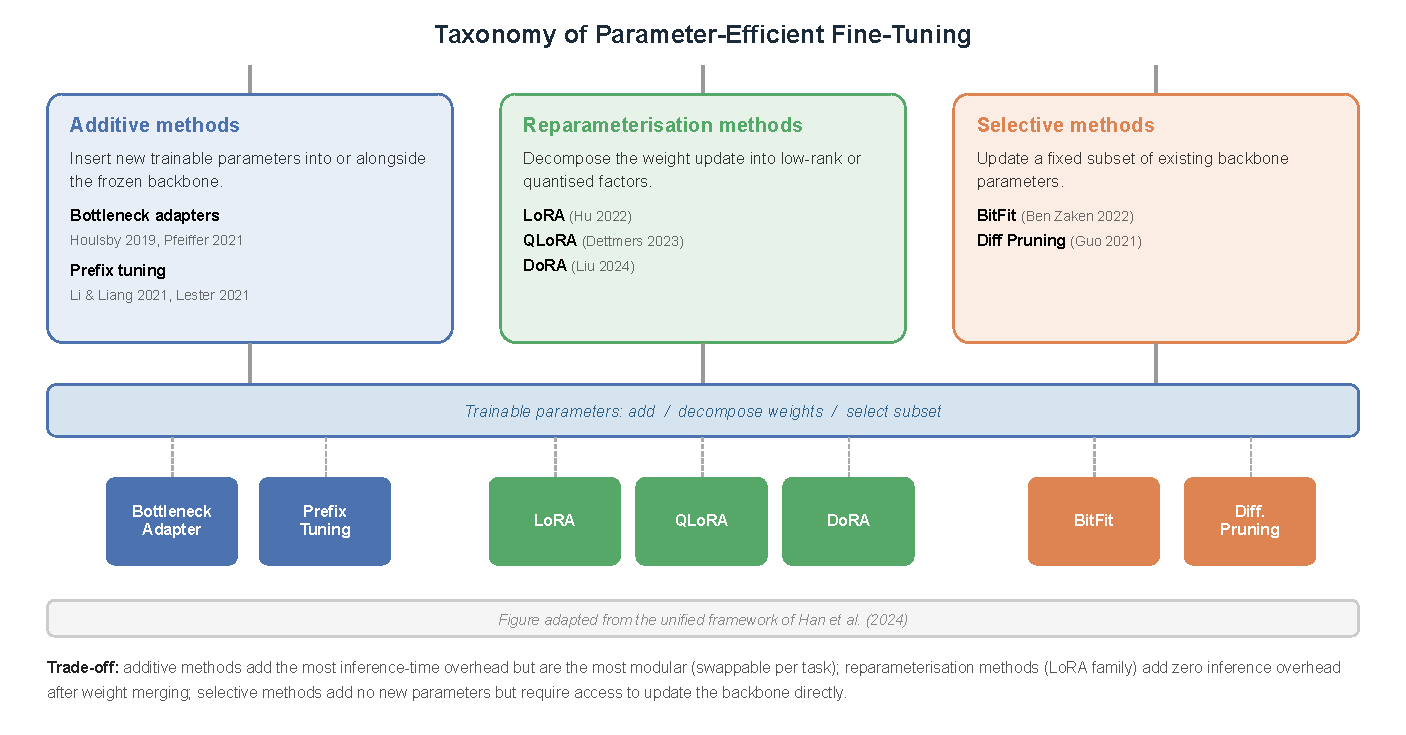
\includegraphics[width=0.85\textwidth]{figures/fig_peft_taxonomy.pdf}
  \caption{Taxonomy of parameter-efficient fine-tuning families (own figure)
    \cite{Han2024}. Additive
    methods (bottleneck adapters, prefix tuning) insert new parameters; reparameterisation
    methods (LoRA, QLoRA) decompose weight updates; selective methods (BitFit)
    update a fixed subset of existing parameters.}
  \label{fig:peft_types}
\end{figure}

\noindent The structural findings of this section are consolidated, alongside the
other four sub-questions, in the centralised discussion in
Section~\ref{sec:synthesis_gap:answers}.
